%!TEX program = xelatex
%!TEX encoding = UTF-8 Unicode

\documentclass[14pt, AutoFakeBold]{ldr}
  

\title{本 科 生 毕 业 答 辩}
\subtitle{利用机器学习进行气体探测器径迹重建的算法研究}

\author{答辩人:王文军}
\institute{指导老师:张毅}
\date{\today}
\titlegraphic{
\includegraphics[height=0.15\textwidth]{lzu_logo.png}}



  



\begin{document}

\maketitle

\AtBeginSection[]
{
  \begin{frame}
    \frametitle{\insertshorttitle}
    \tableofcontents[currentsection,hideallsubsections]
  \end{frame}
}





\section{研究背景}
\subsection{基于裂变时间投影室的新型核裂变测量技术}
\begin{frame}[c]{基于裂变时间投影室的新型核裂变测量技术}
利用机器学习进行\textcolor{red}{气体探测器径迹重建}的算法研究


  \frametitle{基于裂变时间投影室的新型核裂变测量技术}
  \begin{figure}[H]
  \centering
  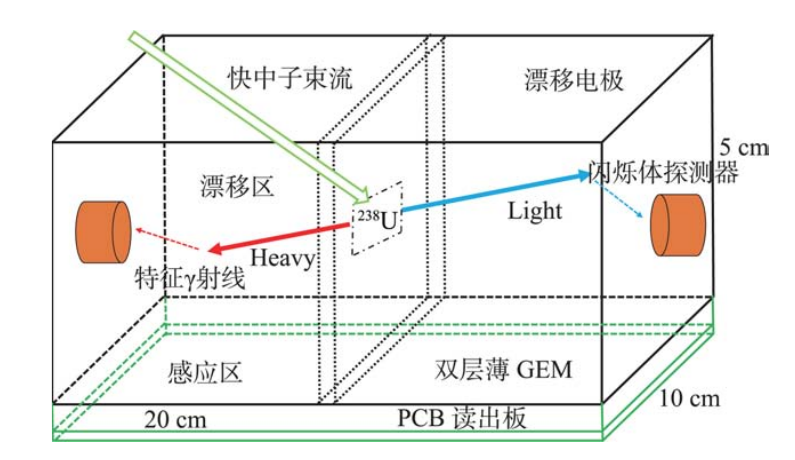
\includegraphics[width=0.9\textwidth]{../figures/GEM-TPC.png}

  \caption{裂变时间投影室探测系统(论文 P6)}
  \label{fig-GEM-TPC}
  \end{figure}
  
\end{frame}



\begin{frame}
  \frametitle{时间投影室的应用}
  \begin{itemize}
    \item 许多大型高能粒子实验都采用其作为中心径迹探测器, 比较著名的有LEP实验的ALEPH, DELPHI, BNL的 STAR, LHC的ALICE等等。
    \item MicroBooNE Collaboration 应用卷积神经网络完成了对时间投影室产生的径迹数据的算法研究。算法包括多粒子径迹图片的分类(Classification)、多粒子径迹图片中的空间定位(Localization)。
    \end{itemize}
\end{frame}



\begin{frame}
  \frametitle{时间投影室的目前的局限}
  \begin{itemize}
    \item 对于裂变碎片的鉴别尚处于空白。
    \item 对于裂变碎片的径迹重建仍然基于经典的离子能损理论。
    \item 如果将径迹简单地拟合为直线无法准确处理这种非线性效应。
    \end{itemize}
  


\end{frame}



\begin{frame}
  \frametitle{每一页内容位置}

  内容老是居中,我想让它居上怎么办?看下一页


\end{frame}




\begin{frame}[t]{每一页内容位置}

  这句话在上面了吧,原因是上面那个[t],默认[c](居中)


\end{frame}



\section{主要内容}

\begin{frame}
  \frametitle{图并排}
  \begin{figure}[H]
    \centering
    
\includegraphics[width=0.3\textwidth]{lzu_logo.png}
  
    \caption{兰州大学(单图)\footnotesize 小字可以这么来}
    \label{fig_lzu}
\end{figure}
  
\end{frame}




\begin{frame}
  \frametitle{图并排}
  \begin{figure}[H]
    \centering
    \subfloat[图1]{
        \label{fig_lzus_0}
        
\includegraphics[width=0.3\textwidth]{lzu_logo.png}
    }
    \subfloat[图2]{
        \label{fig_lzus_1}
        
\includegraphics[width=0.3\textwidth]{lzu_logo.png}
    }\\
    \caption{兰州大学}
    \label{fig_lzus}
\end{figure}
  
\end{frame}


\begin{frame}
  \frametitle{表格}
  \begin{table}[H]
    \centering
    \caption{纳米管参数}
    \begin{tabular}{cccccc} % 控制表格的格式
        \toprule
        参数 & m  & n  & 原子数 & 内径     & 长度    \\
        \midrule
        二硫化钼纳米管  & 15 & 15 & 3420   & 2.3014nm & 11.85nm \\
        碳纳米管  & 16 & 6  & 1112   & 1.5424nm & 6.0nm   \\
        \bottomrule
    \end{tabular}
    \label{tbl_mcnt_nanotube}
\end{table}
\end{frame}

\begin{frame}
\frametitle{左右分栏}
去掉 pause  就不会变成两页了
  \begin{columns}
  \column{0.6\textwidth}

    \begin{itemize}
    \item Ice Age
    \item The Hobbit
    \item The Great Gatsby
    \end{itemize}
  \pause
  \column{0.4\textwidth}
    \begin{itemize}
    \item 冰河世纪
    \item 霍比特人
    \item 了不起的盖茨比
    \end{itemize}
  \end{columns}
\end{frame}





\begin{frame}
  \frametitle{分步动画}


  \onslide<1>{
    第一步显示这一句话,第二步时消失
  }
  \onslide<2,3>{
    \begin{block}{解析:}
      第二、三步显示这一句话
    \end{block}
  }

  \onslide<3>{
    只有第三步显示这一句话
  }

\end{frame}






\section{总结展望}

\begin{frame}
  \frametitle{测试}

  \begin{block}{方框}
    测试一下,参考一篇文献
  \end{block}

\end{frame}





\end{document}